\subsection{Tools Used}
The model was designed using MATLAB\textregisteredmark\ and SIMULINK\textregisteredmark\ R2018B. Analysis was also performed using this software. Additionally, to aid testing, a generic video file was used provided by \hyperlink{https://blogs.unity3d.com/2016/11/28/free-vfx-image-sequences-flipbooks/}{Unity3D}.
\subsection{Assumptions}
The video file used has dimensions of 400x400px. Inside the parameters of certain blocks in the SIMULINK\textregisteredmark\ file this assumption was used and the model will need to be altered to work with video files of other dimensions. Additionally, the input video file was 30fps which is assumed in the frame counter module.
\subsection{Design}
The top level design is shown in Fig. \ref{fig:sysSpecs}. A general overview of this design is presented in this section with in-depth descriptions in later sections.
\begin{figure}[H]
    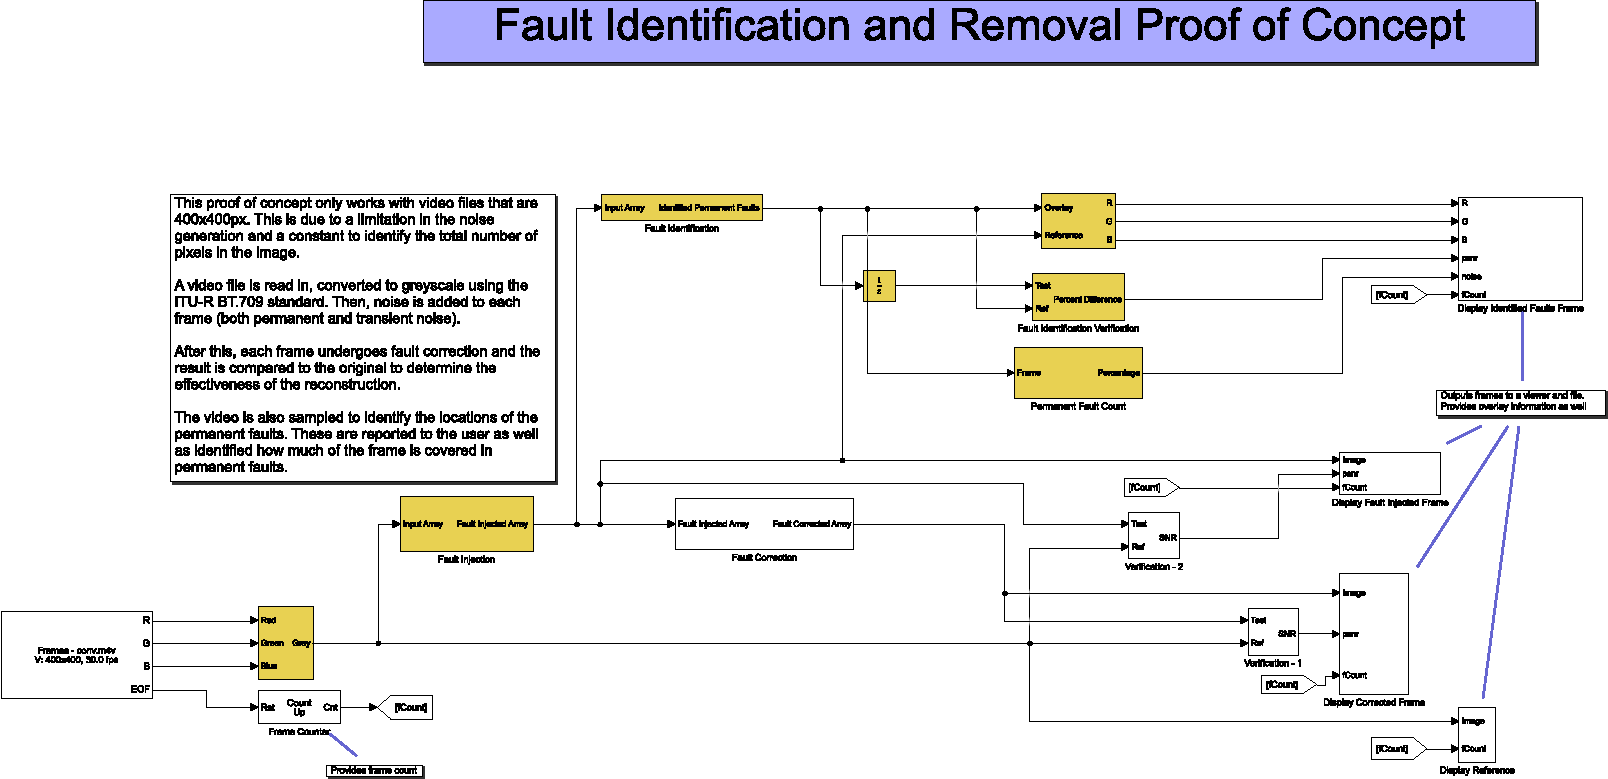
\includegraphics[width=\linewidth]{impl_dsgn}
    \caption{Top Level System Design}
    \label{fig:sysSpecs}
\end{figure}
\par An input video is fed into the \verb!From Multimedia File! block. Each color frame is converted to black and white to make image processing easier. Additionally, the \verb!EOF! output of the \verb!From Multimedia File! is fed into a frame counter's reset port, which is reset every time the video is restarted.
\par From this point, the video is sent to a noise generation unit. Since this model is a proof of concept, it is important to have a reference video as well as a video file with noise added. The noise generation block adds both permanent and transient noise.
\par After the frame has noise added, it is sent to two blocks, one to identify permanent noise in the frame, and another to filter out the noise in the frame.
\par Post noise generation, noise filtering, noise identification, and the reference frames are output to a video display as well as logged to a video file throughout simulation. Frame count information as well as other diagnostic and verification information is overlayed on top of the video frames to aid in analysis.
\subsubsection{ITU-R BT.709 Submodule}
The black and white conversion module follows the ITU-R BT.709 standard for color to black and white conversion. A reproduction of this module along with the coefficients used for each channel is shown in Fig. \ref{fig:btu709}.
\begin{figure}[H]
    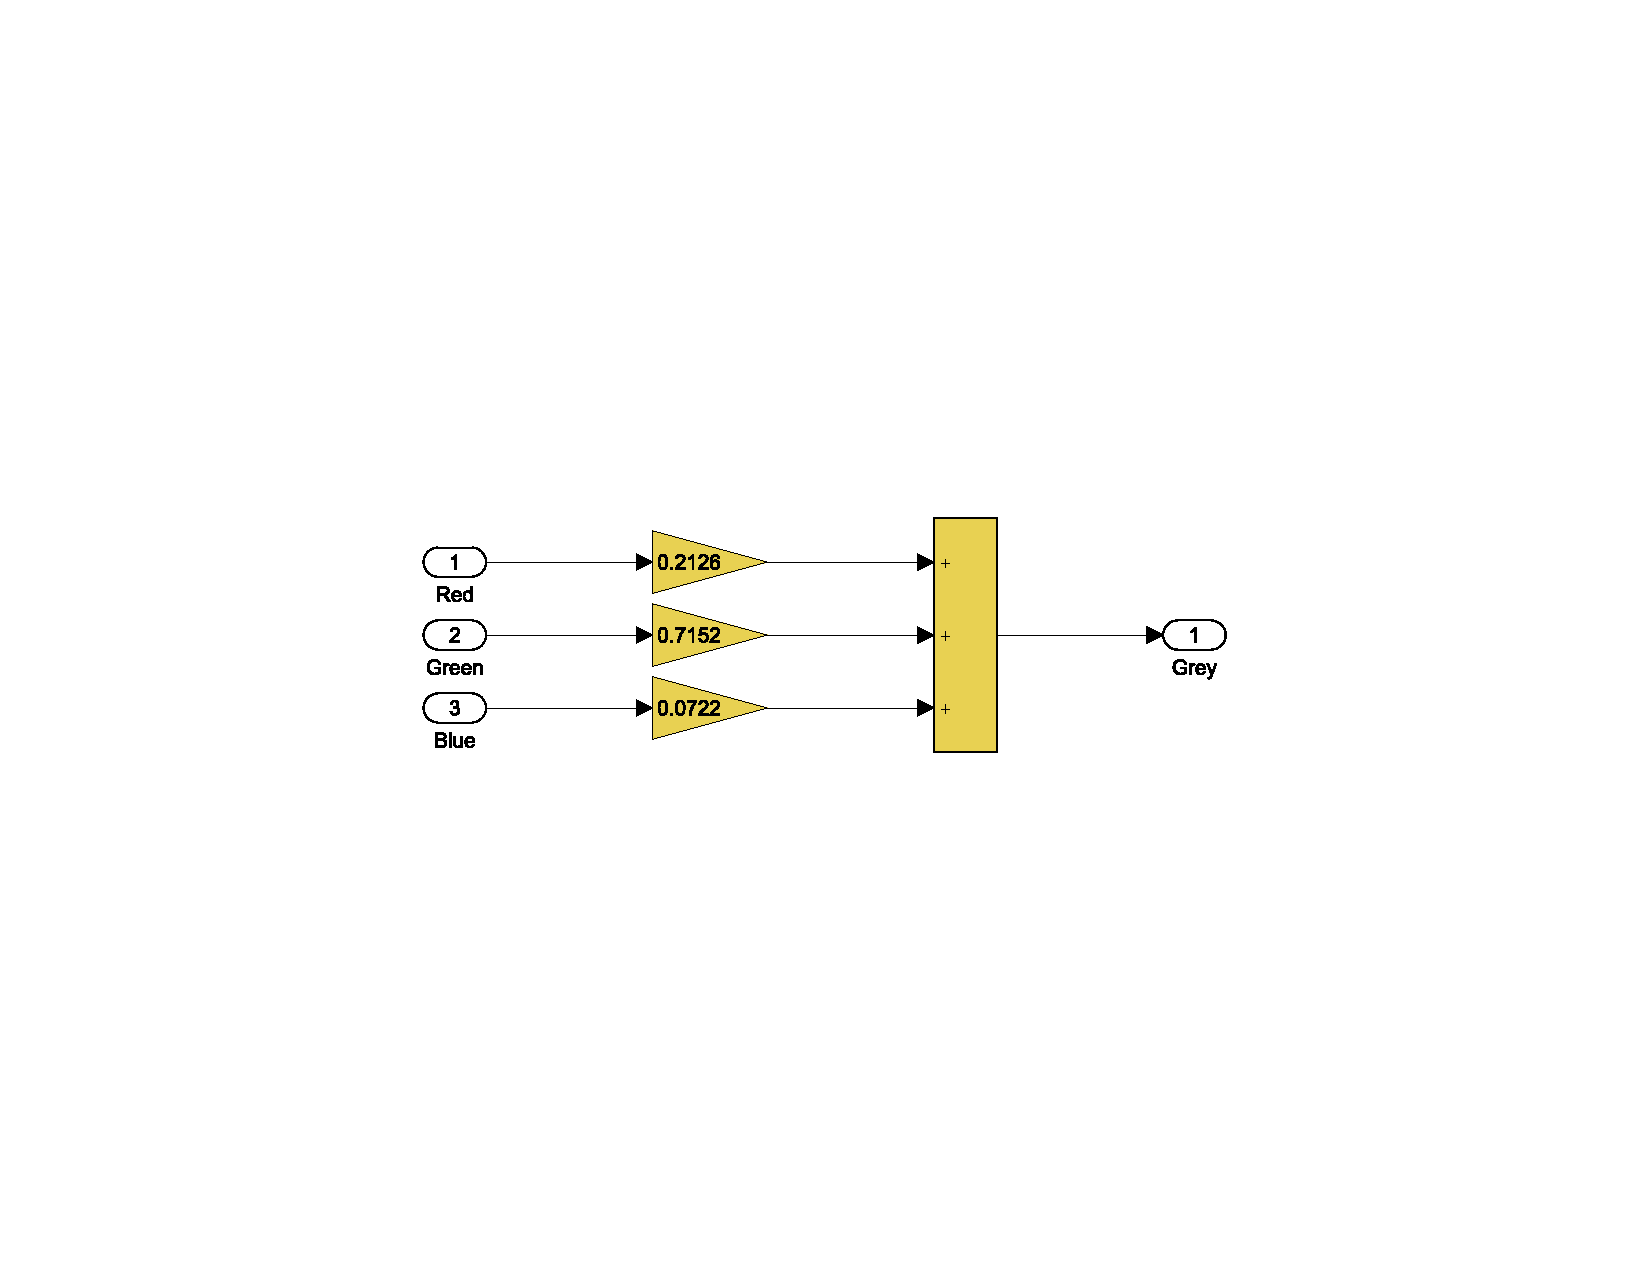
\includegraphics[width=\linewidth]{impl_dsgn_ITU-R BT.709}
    \caption{ITU-R BT.709 Color to Black and White Conversion}
    \label{fig:btu709}
\end{figure}
\subsubsection{Noise Generator}
The Noise generator generates both permanent and transient noise.
\begin{figure}[ht!]
    \subfloat[Top Level Noise Generator Block\label{fig:1a:topLevelNoiseGenerator}]{%
       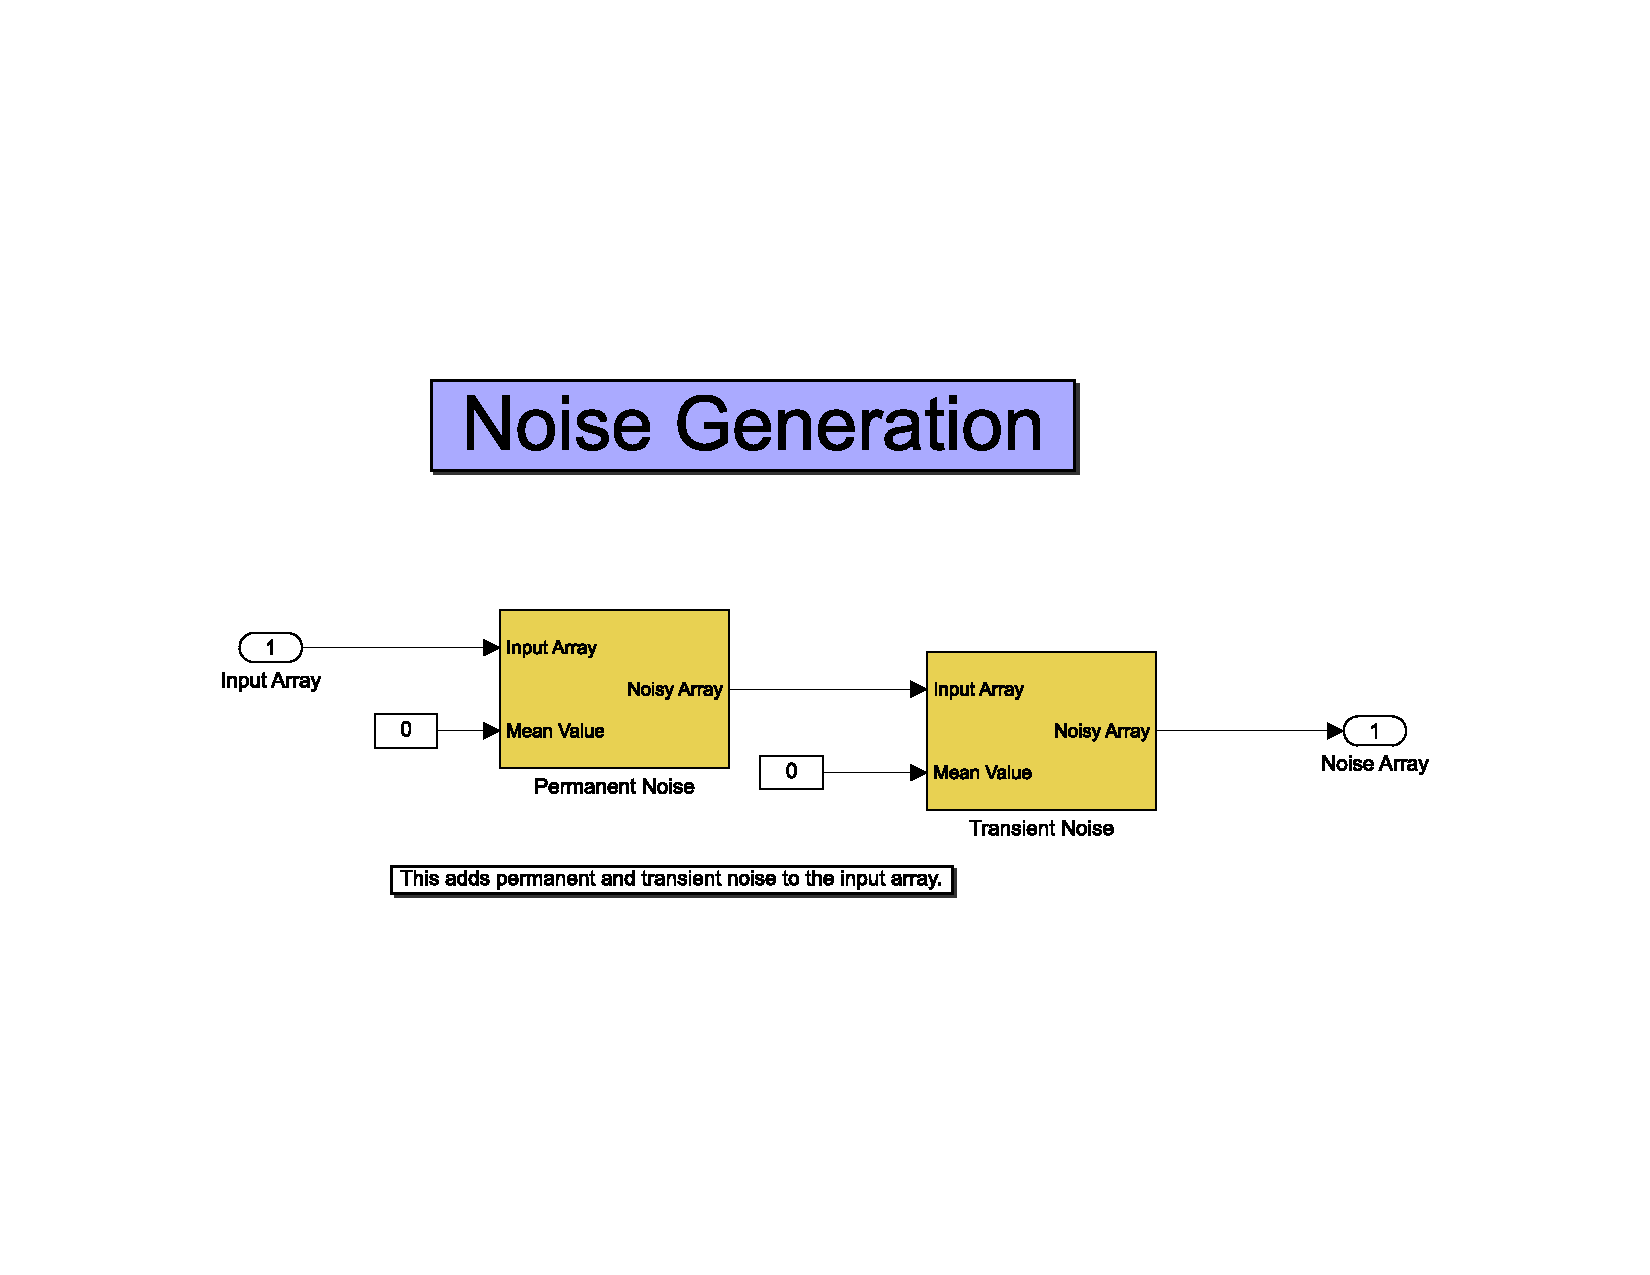
\includegraphics[width=\linewidth]{impl_dsgn_Noise Generator}}
    \\
     \subfloat[Permanent Noise Generator Block\label{fig:1b:permanentNoiseGenerator}]{%
        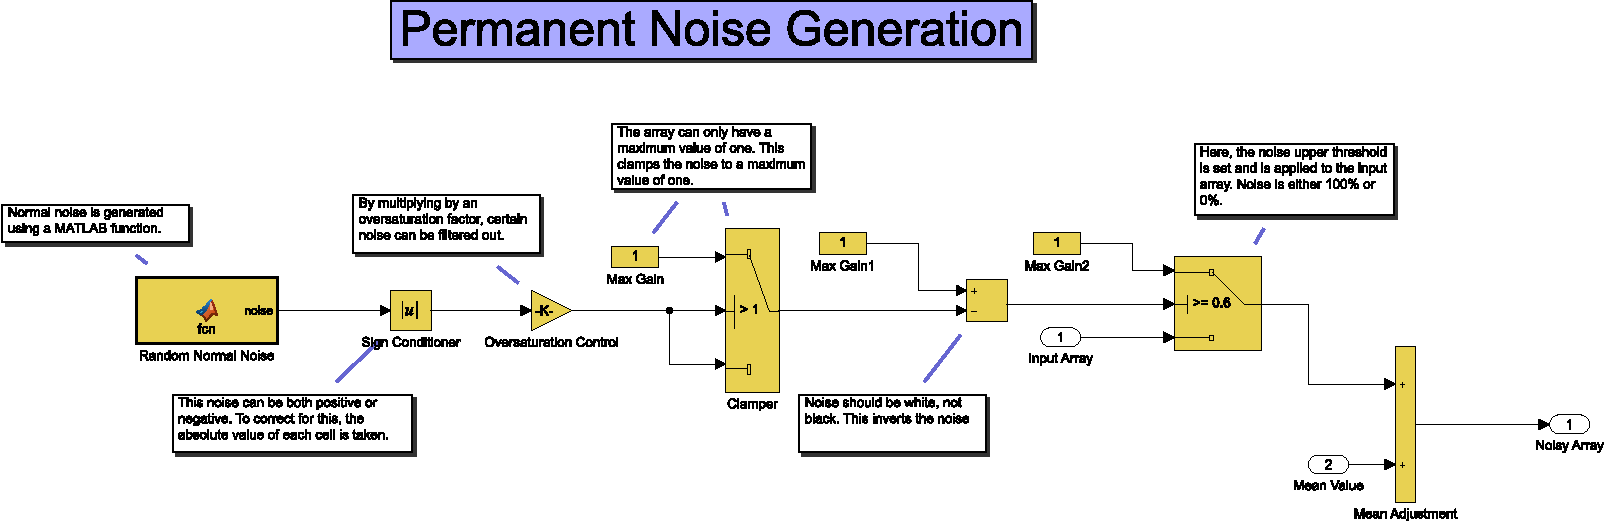
\includegraphics[width=\linewidth]{impl_dsgn_Noise Generator_Permanent Noise}}
    \caption{(a), (b) Shown are the top level noise generator block and the permanent noise generation block. The transient noise generation block is visually identical to the permanent noise generation block. The difference is inside of the MATLAB\textregisteredmark\ function block, and therefore was omitted.}
    \label{fig:noiseGenerator}
\end{figure}
\par As shown in Fig. \ref{fig:1a:topLevelNoiseGenerator}, the reference video frame is fed into the permanent noise generation block and then is fed into the transient noise generation block. Both the transient noise and permanent noise overlays are calculated each frame which results in an decrease in real-time performance of the demo. The transient noise generation block accounted for approximately 67\% of the total execution time followed next by the permanent noise generation block at approximaetly 3.2\% of the total execution time.